\documentclass{beamer}

% To have the citation lists ordered by number.
\usepackage[nocompress]{cite}
\usepackage[utf8]{inputenc}
\usepackage{graphicx}
\usepackage[tight,TABTOPCAP]{subfigure}
\usepackage{amsmath}
\usepackage{amssymb}
\usepackage{amsfonts}
\usepackage{url}
\usepackage{proof}

\usepackage{hyperref}

\usepackage{tikz}
\usepackage{color}

% Allow more than 70% (default) of a page to be filled by figures (100%).
\renewcommand\topfraction{1.0}

%%%%%%%%%% Tool Names %%%%%%%%%%%%
\newcommand{\csisat}{{\sc CSIsat}}
\newcommand{\blast}{{\sc Blast}}
\newcommand{\armc}{{\sc ARMC}}
\newcommand{\mathsat}{{\sc MathSAT}}
\newcommand{\picosat}{{\sc PicoSAT}}
\newcommand{\clpprover}{{\sc CLPprover}}
\newcommand{\foci}{{\sc Foci}}
\newcommand{\sicstus}{{\sc SICStus Prolog}}

%%%%%%%%%% NOTATIONS %%%%%%%%%%%%
\newcommand{\true}{{\it true}}
\newcommand{\false}{{\it false}}
\newcommand{\sat}{{\sc sat}}
\newcommand{\laeuf}{{\sc LA+EUF}}

\renewcommand{\implies}{\Rightarrow}


\mode<presentation>
{
  \usetheme{Warsaw}
  %\usetheme{Frankfurt}
  % or ...

  %\setbeamercovered{transparent}
  % or whatever (possibly just delete it)
  %\setbeamertemplate{footline}[frame number]
  \useoutertheme{mysplit}
}
% Remove the navigation bar
\setbeamertemplate{navigation symbols}{}

\graphicspath{{./imgs/}}

\title[SMT solvers]{SMT solvers, tools of trade in formal methods}

\AtBeginSection[]
{
  \begin{frame}<beamer>
    \frametitle{Outline}
    \tableofcontents[currentsection,hideothersubsections]
  \end{frame}
}

\author{ Damien Zufferey }

\institute{ IST Austria }
\date{\today}

%-------------------------------------------------------------------------
\begin{document}

% Title
\frame[plain]{\titlepage}

\begin{frame}
\tableofcontents
\end{frame}

\section{Introduction}
\begin{frame}
  \frametitle{What are SMT solvers ?}
  SMT Solver are tools that tell if a given formula has some solution.

  \vspace{20pt}

  For instance:
  \begin{center}
    $p = f(x + a) ~\land~ q = f( y + b ) ~\land~ a = b ~\land$\\
    $s = f(p + c)  ~\land~ t = f(q + d)  ~\land~ c = d ~\land$\\
    $1 = s -t + z ~\land~ x = y ~\land~ z = 0$
  \end{center}
  in unsatisfiable.

  
\end{frame}

\begin{frame}
  \frametitle{Challenges}
  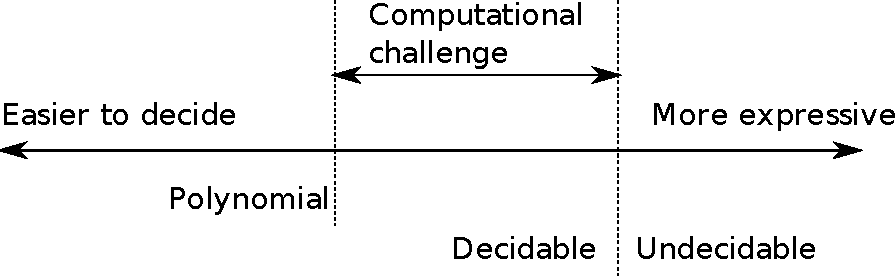
\includegraphics[scale=0.72]{challenge}
\end{frame}

\section{Formalism}
\subsection{General Concepts}
\begin{frame}
  \frametitle{Propositional Logic (PL)}
  Also known as boolean logic.
  \begin{block}{Syntax}
  $F :: ~~ F \wedge F ~~|~~ F \vee F ~~|~~ \neg F ~~|~~ \top ~~|~~ \bot ~~|~~ \mathit{propositional\ variable} $
  \end{block}
  Other operators ($\rightarrow, \leftrightarrow, \oplus$) are syntactic sugar.

  \begin{block}{Semantics}
  An interpretation $I$ is an assignment of the propositional variables to either $\top$ or $\bot$,
  i.e. $I = \{P \mapsto \top, Q \mapsto \bot, \ldots \}$
  \end{block}
\end{frame}

\begin{frame}
  \frametitle{Propositional Logic: example}
  You need to schedule 3 talks given by 3 different speakers with their own availability.

  \vspace{10pt}

  Create 9 variables $x_{ws} ~ (w \in 1..3, s \in 1..3)$.\\
  For each speaker $s$, add $\neg x_{ws}$ where $w$ corresponds to the dates where $s$ in not available.\\
  For each speaker $s$, add $x_{is} \rightarrow \neg x_{js} \wedge \neg x_{ks}$ with $i,j,k$ all different.\\
  For each week $w$, add $x_{w1} \lor x_{w2} \lor x_{w3}$.\\
  For each week $w$, add $x_{wi} \rightarrow \neg x_{wj} \wedge \neg x_{wk}$ with $i,j,k$ all different.\\
  
\end{frame}

\begin{frame}
  \frametitle{First Order Logic (FOL)}
  \begin{block}{Syntax}
  $T :: ~~ \mathit{constants} ~~|~~ \mathit{variables} ~~|~~ \mathit{functions} $\\
  $P :: ~~ \mathit{predicate} ~~|~~ \mathit{propositional\ variables} ~~|~~ \top ~~|~~ \bot $\\
  $F :: ~~ P ~~|~~ F \wedge F ~~|~~ F \vee F ~~|~~ \neg F ~~|~~ \exists x. F[x] ~~|~~ \forall x. F[x]$
  \end{block}
  Example: $\forall x. p(f(x), x) \rightarrow (\exists y. p(g(x,y), g(y,x)))$
  \begin{block}{Semantics}
  An interpretation $I = \langle D, \alpha \rangle$ is a pair domain, assignment.
  $D$ is a non-empty set of values.
  $\alpha$ maps variables and constants to elements of $D$,
  $n$-ary functions to functions over $D^n \rightarrow D$,
  and $n$-ary predicates to predicates over $D^n \rightarrow \{true, false\}$.
  \end{block}
  Interpretations are also known as models.
\end{frame}

\begin{frame}
  \frametitle{Quantifiers and free variables}
  Free variables are either universally or existentially quantified, depending on the problem we are solving:

  \begin{itemize}
  \item The universal closure ($\forall$) for the validity problem.
  \item The existential closure ($\exists$) for the satisfiability problem.
  \end{itemize}
\end{frame}

\subsection{First Order Theories}
\begin{frame}
  \frametitle{First Order Theories}
  \begin{block}{Definition}
  A theory $T = \langle \Sigma, \mathcal{A} \rangle$ is a pair signature, axioms.
  \begin{itemize}
  \item $\Sigma$ is a set of constants, functions and predicates symbols.
  \item $\mathcal{A}$ is a set of closed FOL formula over the elements of $\Sigma$.
  \end{itemize}
  \end{block}

  The quantifier-free fragment of a theory (QFF) is a syntactic restriction that prevents using quantifiers in formulas.
  
  The conjunctive QFF (CQFF) is the fragment where formulas are only conjunctions.
\end{frame}

\begin{frame}
  \frametitle{Equality with Uninterpreted Function symbols (EUF)}
  Example: $f(f(f(f(f(a))))) = a \land f(f(f(a))) = a \land f(a) \neq a$

  \vspace{10pt}

  Signature: $\Sigma_{EUF} = \{ =, a, b, c, \ldots, f, g, h, \ldots, p, q, r, \ldots \}$\\
  Axioms:
  \begin{enumerate}
  \item $\forall x. x = x$ \hfill (reflexivity)
  \item $\forall x, y. x = y \rightarrow y = x$ \hfill (symmetry)
  \item $\forall x, y, z. x = y \land y = z \rightarrow x = z$ \hfill (transitivity)
  \item for all $n$-ary function symbol $f$:
    $\forall \vec x, \vec y. \left( \bigwedge_{i=1}^n x_i = y_i \right) \rightarrow f(\vec x) = f(\vec y)$
    \hfill (function congruence)
  \item for all $n$-ary predicates symbol $p$:
    $\forall \vec x, \vec y. \left( \bigwedge_{i=1}^n x_i = y_i \right) \rightarrow p(\vec x) \leftrightarrow p(\vec y)$
    \hfill (predicate congruence)
  \end{enumerate}
\end{frame}

\begin{frame}
  \frametitle{Presburger Arithmetic($\mathbb{N}$), Theory of Integers ($\mathbb{Z}$)}
  Example: $ \forall w,x.~ \exists y,z.~ x + 2 y - z -13 > - 3 w + 5$

  \vspace{10pt}

  Signature: $\Sigma_{\mathbb{N}} = \{ 0, 1, +, =\}$\\
  Axioms:
  \begin{enumerate}
  \item $\forall x. \neg(x + 1 = 0)$ \hfill (zero)
  \item $\forall x, y. x+1 = y+1 \rightarrow x = y$ \hfill (successor)
  \item $F[0] \land (\forall x. F[x] \rightarrow F[x+1]) \rightarrow \forall x. F[x]$ \hfill (induction) 
  \item $\forall x. x + 0 = x$ \hfill (plus zero)
  \item $\forall x, y. x+(y+1) = (x+y)+1 $ \hfill (plus successor)
  \end{enumerate}

\end{frame}

\begin{frame}
  \frametitle{Theory of Reals ($\mathbb{R}$), Theory of Rationals ($\mathbb{Q}$)}
  Signature: $\Sigma_{\mathbb{R}} = \{ 0, 1, +, \cdot, =, \geq\}$\\
  Axioms: ...

  \vspace{10pt}

  Signature: $\Sigma_{\mathbb{Q}} = \{ 0, 1, +, -, =, \geq\}$\\
  Axioms: ...
\end{frame}


\begin{frame}
  \frametitle{Linear Arithmetic (LA), Difference Logic (DL)}
  LA and DL are fragments of the theories of $\mathbb{N,Z,Q,R}$.
  
  \begin{description}
  \item[LA] has terms of the form $\sum_i a_i x_i \geq b$.\\
    e.g. $3 x + 2 y \leq 5 z  \land 2 x - 2 y = 0$

  \item[DL] has terms of the form $ x - y \geq c$.\\
    e.g. $x < y + 5 \land y \leq 4 \land x = z - 1$
  \end{description}
\end{frame}

\section{Algorithm}
\subsection{Propositional Logic}
\begin{frame}
  \frametitle{DPLL: definition}
  We are searching a solution for $P \land (\neg P \lor Q) \land (R \lor \neg Q \lor S)$.

  \vspace{10pt}

  Assumption: formula in conjunctive normal form (CNF): $\bigwedge_i \bigvee_j x_{ij}$.\\
  A \alert{literal} is a variable or its negation.\\
  A disjunction of literals is a \alert{clause}.

  \vspace{10pt}

  An \alert{unit} clause is a clause containing \alert{only one literal}.\\
  To satisfy the unit clause $(P)$, $P$ has to be assigned to true.

\end{frame}

\begin{frame}
  \frametitle{DPLL: algorithm}

  unit resolution (boolean constraint propagation): \[\infer{C[\bot]}{l & C[\neg l]}\]

  case splitting: \[ F[x] \leftrightarrow F[\bot] \lor F[\top] \]
  
  \begin{block}{Algorithm}
  \centering
  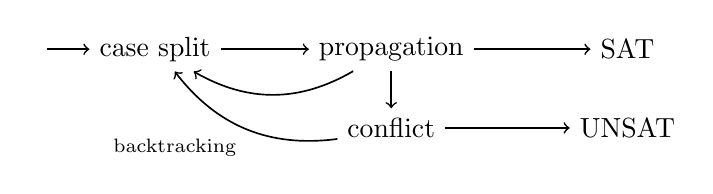
\begin{tikzpicture}[semithick, ->]
  \node  (o) at (-1.5,0) {};
  \node  (a) at (0,0) {case split};
  \node  (b) at (3,0) {propagation};
  \node  (c) at (3,-1) {conflict};
  \node  (d) at (6,0) {SAT};
  \node  (e) at (6,-1) {UNSAT};
  \path  (o) edge (a)
         (a) edge (b)
         (b) edge (c)
         (b) edge (d)
         (c) edge (e)
         (b) edge[bend left] (a)
         (c) edge[bend left] node[below left] {{\scriptsize backtracking}} (a);
  \end{tikzpicture}
  \end{block}
\end{frame}
%TODO example

\begin{frame}
  \frametitle{DPLL: learning}
  While backtracking it is possible to learn new clauses by resolution:
  \[\infer{Q \lor R}{P \lor Q & \neg P \lor R}\]

  \vspace{10pt}

  Example: $(P \lor Q) \land (\neg P \lor Q) \land (P \lor \neg Q) \land (\neg P \lor \neg Q)$.
\end{frame}

\begin{frame}[1-7]
  \frametitle{DPLL: example}
  \begin{center}

  \textcolor{red}{
  \alt<2>{$P \mapsto \top$}{
  \alt<3>{$Q \mapsto \top$}{
  \alt<4>{backtracking}{
  \alt<5>{$P \mapsto \bot$}{
  \alt<6>{$Q \mapsto \top$}{
  \alt<7>{ backtracking }{  }
  }}}}}}

  \vspace{10pt}

  $
    \visible<1,4,5,7->{(\invisible<5>{P \lor} Q)}
    \visible<1,4,5,7->{\land}
    \visible<1-2,4,7->{(\visible<1,4->{\neg P \lor} Q)}
    \visible<1-2,4,7->{\land}
    \visible<1,4->{(\invisible<5-6>{P \lor} \alt<6>{\bot}{\neg Q})}
    \visible<1,4,7->{\land}
    \visible<1-4,7->{(\visible<1,4->{\neg P \lor} \alt<3>{\bot}{\neg Q})}
  $
  \end{center}

  \vspace{10pt}

  \[
  \infer{\visible<7->{\bot}}{
    \visible<7->{
    \infer{P}{
      (P \lor Q)
      &
      (P \lor \neg Q)
    }
    }
    &
    \visible<4->{
    \infer{\neg P}{
      (\neg P \lor Q)
      &
      (\neg P \lor \neg Q)
    }
    }
  }
  \]
\end{frame}

\begin{frame}
  \frametitle{DPLL: Decision policy}
    Most of the generated sat problems are \alert{structured}.
    The goal of a SAT solver is to quickly figure out what is important.
    The role of the decision policy is to guess which variables are important.

  \vspace{10pt}

    A good decision policy and learning is the key to scaling to problems with thousands of variables.

\end{frame}

\subsection{Equality with Uninterpreted Function symbols}
\begin{frame}
  \frametitle{EUF: Example}
  \begin{center}
  $f(f(f(f(f(a))))) = a \land f(f(f(a))) = a \land \alert<4>{f(a) \neq a}$
  \end{center}

  \vspace{10pt}

  Satisfiable or not ?
  \begin{itemize}
  \item<2-> $f(f(a)) = a$
  \item<3-> \alert<4>{$f(a) = a$}
  \end{itemize}
\end{frame}

\begin{frame}
  \frametitle{EUF: Congruence Closure}
  
  \begin{tikzpicture}[remember picture, overlay, semithick, ->, node distance=1cm]
  \node [draw,circle,xshift=-2cm,yshift=1.5cm] (f5) at (current page.east) {$f$};
  \node [draw,circle] (f4) [below of=f5] {$f$};
  \node [draw,circle] (f3) [below of=f4] {$f$};
  \node [draw,circle] (f2) [below of=f3] {$f$};
  \node [draw,circle] (f1) [below of=f2] {$f$};
  \node [draw,circle] (a)  [below of=f1] {$a$};
  \path  (f5) edge (f4)
         (f4) edge (f3)
         (f3) edge (f2)
         (f2) edge (f1)
         (f1) edge (a);
  \visible<2->{
  \path  (f5) edge [red, bend left] (a)
         (f3) edge [red, bend left] (a);
  }
  \visible<3->{
  \path  (a) edge [blue, bend left] (f1)
         (a) edge [blue, bend left] (f2)
         (a) edge [blue, bend left] (f3)
         (a) edge [blue, bend left] (f4)
         (a) edge [blue, bend left] (f5);
  \path  (f1) edge [blue, bend left] (f2)
         (f1) edge [blue, bend left] (f3)
         (f1) edge [blue, bend left] (f4)
         (f1) edge [blue, bend left] (f5);
  \path  (f2) edge [blue, bend left] (f3)
         (f2) edge [blue, bend left] (f4)
         (f2) edge [blue, bend left] (f5);
  \path  (f4) edge [blue, bend left] (f5);
  }
  \end{tikzpicture}

  \parbox{6cm}{
  DAG representing the terms:\\
  $\{a, f(a), f(f(a)), f^3(a), f^4(a), f^5(a)\}$

  \vspace{10pt}

  \visible<2->{
  Union-find data structure:\\
  The nodes keep a pointer to the \textcolor{red}{representative} of their equivalence class.
  }

  \vspace{10pt}

  \visible<3->{
  The representative of an equivalence class keeps pointers to its \textcolor{blue}{congruence closure parents}.
  }
  }

\end{frame}

\begin{frame}
  \frametitle{Congruence Closure: example}
  
  \begin{tikzpicture}[remember picture, overlay, semithick, ->, node distance=1cm]
  \node [draw,circle,xshift=-2cm,yshift=1.5cm] (f5) at (current page.east) {$f$};
  \node [draw,circle] (f4) [below of=f5] {$f$};
  \node [draw,circle] (f3) [below of=f4] {$f$};
  \node [draw,circle] (f2) [below of=f3] {$f$};
  \node [draw,circle] (f1) [below of=f2] {$f$};
  \node [draw,circle] (a)  [below of=f1] {$a$};
  \path  (f5) edge (f4)
         (f4) edge (f3)
         (f3) edge (f2)
         (f2) edge (f1)
         (f1) edge (a);

  \visible<2->{\path  (f3) edge [red, bend left] (a);}
  \visible<3->{\path  (f4) edge [red, bend left] (f1);}
  \visible<4->{\path  (f5) edge [red, bend left] (f2);}
  \visible<5->{\path  (f2) edge [red, bend left] (a);}
  \visible<6->{\path  (a) edge [red, bend right] (f1);}

  \invisible<6->{
  \path  (a) edge [blue, bend left] (f1)
         (a) edge [blue, bend left] (f2)
         (a) edge [blue, bend left] (f3)
         (a) edge [blue, bend left] (f4)
         (a) edge [blue, bend left] (f5);
  }
  \visible<6->{
  \path  (f1) edge [blue, loop left] (f1);
  }

  \path  (f1) edge [blue, bend left] (f2)
         (f1) edge [blue, bend left] (f3)
         (f1) edge [blue, bend left] (f4)
         (f1) edge [blue, bend left] (f5);

  \invisible<5->{
  \path  (f2) edge [blue, bend left] (f3)
         (f2) edge [blue, bend left] (f4)
         (f2) edge [blue, bend left] (f5);
  }
  
  \invisible<2->{
  \path  (f3) edge [blue, bend left] (f4)
         (f3) edge [blue, bend left] (f5);
  }
  
  \invisible<3->{
  \path  (f4) edge [blue, bend left] (f5);
  }
  \end{tikzpicture}
  
  \parbox{6cm}{
  \begin{itemize}
  \item<2-> adding $f^3(a) = a$
  \item<3-> congruence $f^4(a) = f(a)$
  \item<4-> congruence $f^5(a) = f^2(a)$
  \item<5-> adding $f^5(a) = a$
  \item<6-> congruence $f^3(a) = f(a)$
  \item<7-> conflict with $f(a) \neq a$
  \end{itemize}
  }
\end{frame}

\subsection{Difference Logic}
\begin{frame}
  \frametitle{Difference Bound Matrices (1)}
  $x \leq y + 5 ~\land~ y \leq 4 ~\land~ x = z - 1$\\
  \vspace{5pt}
  rewritten as a DL formula:\\
  \vspace{5pt}
  $x -y \leq 5 ~\land~ y - x_0 \leq 4 ~\land~ x - z \leq - 1 ~\land~ z - x \leq 1$\\
  \vspace{5pt}
  as a graph:

  \begin{figure}
  \centering
  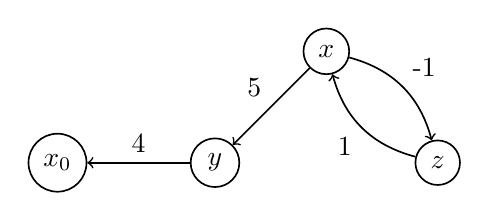
\begin{tikzpicture}[semithick, ->, node distance=2cm]
  \node [draw,circle] (x) at (0,0) {$x$};
  \node [draw,circle] (y) [below left of=x] {$y$};
  \node [draw,circle] (z) [below right of=x] {$z$};
  \node [draw,circle] (x0) [left of=y] {$x_0$};

  \path  (x) edge node [above left] {5} (y)
         (y) edge  node [above] {4}  (x0)
         (x) edge [bend left]  node [above right] {-1} (z)
         (z) edge [bend left]  node [below left] {1} (x);
  \end{tikzpicture}
  \end{figure}

\end{frame}

\begin{frame}
  \frametitle{Difference Bound Matrices (2)}
  $
      \alert<2>{x - y \leq 3}
    ~\land~
      \alert<2>{y - z \leq -5}
    ~\land~
      x - z \leq - 1
    ~\land~
      \alert<2>{z - x \leq 1}
  $\\
  \vspace{5pt}
  as a graph:

  \begin{figure}
  \centering
  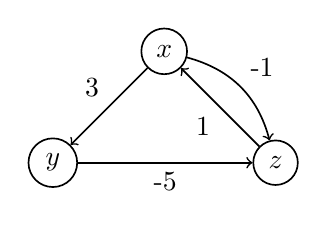
\begin{tikzpicture}[semithick, ->, node distance=2cm]
  \node [draw,circle] (x) at (0,0) {$x$};
  \node [draw,circle] (y) [below left of=x] {$y$};
  \node [draw,circle] (z) [below right of=x] {$z$};

  \alert<2>{
  \path  (x) edge node [above left] {3} (y)
         (y) edge  node [below] {-5} (z)
         (z) edge node [below left] {1} (x);
  }
  \path  (x) edge [bend left]  node [above right] {-1} (z);
  \end{tikzpicture}
  \end{figure}

  \visible<2->{
      $x - y + y - z + z - x \leq 3 -5 +1 ~~ \leftrightarrow ~~ 0 \leq -1 $\\
      \vspace{5pt}
      The formula is satisfiable iff there is no negative cycle.
  }

\end{frame}

\subsection{Linear Arithmetic}
\begin{frame}
  \frametitle{Simplex ($\mathbb{Q,R}$)}
  \begin{center}
  $ 2 x - y \geq 0 ~\land~ - x + 2 y \geq 0 ~\land~ x + y \geq 2 $

  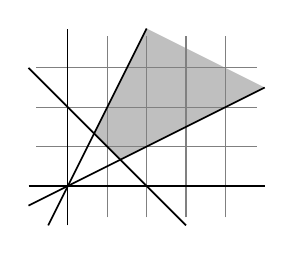
\begin{tikzpicture}[semithick]
    \begin{scope}
    \draw[step=.5cm,gray,thin] (-0.4,-0.4) grid (2.4,1.9);
    \draw[thin] (-0.5,0) -- (2.5,0);
    \draw[thin] (0,-0.5) -- (0,2);

    \pgfsetfillopacity{0.5}
    \fill[gray] (0.666,0.333) -- (0.333,0.666) -- (1,2) -- (2.5,1.25);
    \pgfsetfillopacity{1}
    \draw (-0.5,1.5) -- (1.5,-0.5);
    \draw (-0.5,-0.25) -- (2.5,1.25);
    \draw (-0.25,-0.5) -- (1,2);
    \end{scope}
  \end{tikzpicture}
  \end{center}
    
  Wlog such a problem can be written as $A \vec x \geq \vec b$.\\
  \vspace{5pt}
  Introducing one slack variable per constraint we get:\\
  $A' \vec x' = 0 ~\bigwedge_{i=1}^m l_i \leq s_i \leq u_i$
  ~~where~
  $A' = [A I_m], \vec x' = [\vec x \vec s]$

  %Define system in Matrix form, slack variables.
  %explain what is a basis, a feasible basis.
  %a basis is easy to solve (square matrix)
  %Optimisation problem (phase 1)
\end{frame}

\begin{frame}
  \frametitle{Simplex ($\mathbb{Q,R}$)}
  $\begin{array}{lclc} 2 x - y & \geq & 0 & \land \\ - x + 2 y & \geq & 0  & \land \\ x + y & \geq & 2  & \end{array}$
  ~~{\Huge $\Rightarrow$}~~
  $\begin{array}{rclc}
    2 x - y - s_1 & = & 0 & \land \\
    - x + 2 y - s_2 & = & 0  & \land \\
    x + y - s_3 & = & 0  & \land \\
    s_1 & \geq & 0 & \land \\ 
    s_2 & \geq & 0 & \land \\ 
    s_3 & \geq & 2 
  \end{array}$

  \vspace{10pt}
  
  $
  A =\left(\begin{array}{cc} 2 & -1 \\ -1 & 2 \\ 1 & 1 \end{array}\right)
  $
  ~~{\Huge $\Rightarrow$}~~
  $
  A' =\left(\begin{array}{ccccc}
    2 & -1 & -1 & 0 & 0 \\ 
    -1 & 2 & 0 & -1 & 0 \\
    1 & 1 & 0 & 0 & -1
  \end{array}\right)
  $
  %\left(\begin{array}{c} x \\ y \end{array}\right)
\end{frame}

\begin{frame}
  \frametitle{Simplex ($\mathbb{Q,R}$)}
  $
  \left(\begin{array}{ccccc}
    \invisible<2>{2}  & \invisible<2,3-4>{-1} & -1 & \invisible<5->{0}  & \invisible<3->{0} \\ 
    \invisible<2>{-1} & \invisible<2,3-4>{2}  & 0  & \invisible<5->{-1} & \invisible<3->{0} \\
    \invisible<2>{1}  & \invisible<2,3-4>{1}  & 0  & \invisible<5->{0}  & \invisible<3->{-1}
  \end{array}\right)
  =
  \left(\begin{array}{c}
    0 \\ 
    0 \\
    \alt<3->{\alert<3>{2}}{0}
  \end{array}\right)
  $
  \hfill
  $
  \begin{array}{rcl}
    s_1 & \geq & 0 \\ 
    \alert<4>{s_2} & \alt<-4>{\geq}{=} & \alert<4>{0} \\ 
    \alert<2>{s_3} & \alt<-2>{\geq}{=} & \alert<2>{2}
  \end{array}
  $

  \vspace{10pt}

  \begin{center}
  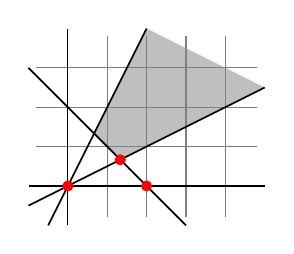
\begin{tikzpicture}[semithick]
    \begin{scope}
    \draw[step=.5cm,gray,thin] (-0.4,-0.4) grid (2.4,1.9);
    \draw[thin] (-0.5,0) -- (2.5,0);
    \draw[thin] (0,-0.5) -- (0,2);

    \pgfsetfillopacity{0.5}
    \fill[gray] (0.666,0.333) -- (0.333,0.666) -- (1,2) -- (2.5,1.25);
    \pgfsetfillopacity{1}
    \draw (-0.5,1.5) -- (1.5,-0.5);
    \draw (-0.5,-0.25) -- (2.5,1.25);
    \draw (-0.25,-0.5) -- (1,2);
    \visible<2>{\fill[red] (0,0) circle (2pt);}
    \visible<3-4>{\fill[red] (1,0) circle (2pt);}
    \visible<5>{\fill[red] (0.666,0.333) circle (2pt);}
    \end{scope}
  \end{tikzpicture}
  \end{center}
\end{frame}

\begin{frame}
  \frametitle{Simplex ($\mathbb{N}$)}
  Branch-and-bound method:
    \begin{itemize}
      \item solve the \emph{relaxed} linear problem (solution in $\mathbb{R}^n$)
      \item \emph{branch} on non-integral variables ($\leq \lfloor x \rfloor ~\lor~ \lceil x \rceil \leq$)
    \end{itemize}

  \vspace{10pt}
  
  \begin{center}
  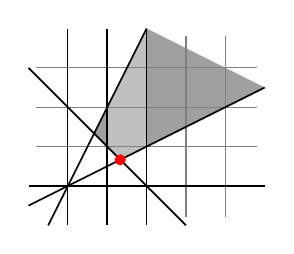
\begin{tikzpicture}[semithick]
    \begin{scope}
    \draw[step=.5cm,gray,thin] (-0.4,-0.4) grid (2.4,1.9);
    \draw[thin] (-0.5,0) -- (2.5,0);
    \draw[thin] (0,-0.5) -- (0,2);

    \pgfsetfillopacity{0.5}
    \visible<-2>{\fill[gray] (0.666,0.333) -- (0.333,0.666) -- (1,2) -- (2.5,1.25);}
    \visible<3->{
      \fill[gray] (0.5,0.5) -- (0.333,0.666) -- (0.5,1);
      \fill[gray] (1,0.5) -- (1,2) -- (2.5,1.25);
      \pgfsetfillopacity{1}
      \draw (0.5,-0.5) -- (0.5,2);
      \draw (1,-0.5) -- (1,2);
    }
    \pgfsetfillopacity{1}
    \draw (-0.5,1.5) -- (1.5,-0.5);
    \draw (-0.5,-0.25) -- (2.5,1.25);
    \draw (-0.25,-0.5) -- (1,2);
    \visible<2>{\fill[red] (0.666,0.333) circle (2pt);}
    \end{scope}
  \end{tikzpicture}
  \end{center}

\end{frame}

\section{SMT Solver}

\subsection{Combining Theories}
\begin{frame}
  \frametitle{Nelson-Oppen (T$_1$ + T $_2$): requirements}
  \begin{block}{Idea}
  T$_1$, T$_2$ share the `=' symbol.
  Propagating equality constraints across the theories is sufficient to derive contradictions.
  \end{block}

  \vspace{10pt}
  
  Requirements:
  \begin{itemize}
  \item T$_1$, T$_2$ are quantifier-free first-order theories with equality.
  \item $\Sigma_1 \cap \Sigma_2 = \{=\}$
  \item There are decision procedure for T$_1$ and T$_2$.
  \item T$_1$, T$_2$ are interpreted over an infinite domain (stably infinite).
  \item \emph{optionally} T$_1$, T$_2$ are convex theories.
  \end{itemize}
\end{frame}

\begin{frame}
  \frametitle{Nelson-Oppen (T$_1$ + T $_2$): convex theory}
  Consider a CQF formula $F$ and a disjunction $\bigvee_{i=1}^n u_i = v_i$.

  The theory T is convex if
  \[
    \left( F \rightarrow \bigvee_{i=1}^n u_i = v_i \right)
    ~\rightarrow~ (F \rightarrow u_k = v_k) ~\text{for some $k \in \{1..n\}$}
  \]
  
\end{frame}

\begin{frame}
  \frametitle{Nelson-Oppen (T$_1$ + T $_2$): purification}
  \begin{center}
  $f(x_1, 0) \geq x_3 ~\land~ f(x_2,0) \leq x_3 ~\land$\\
  $x_1 \geq x_2 ~\land~ x_2 \geq x_1 ~\land~ x_3 - f(x_1, 0) \geq 1$

  \vspace{10pt}

  \begin{tabular}{l | l}
  F$_1$ (LA($\mathbb{Q}$)) & F$_2$ (EUF)\\
  \hline
  $a_1 \geq x_3$  &  $a_1 = f(x_1, a_0)$ \\
  $a_2 \leq x_3$  &  $a_2 = f(x_2, a_0)$ \\
  $x_1 \geq x_2$  & \\
  $x_2 \geq x_1$  & \\
  $x_3 - a_1 \geq 1$  & \\
  $a_0 = 0$  & \\
  \end{tabular}
  \end{center}
\end{frame}

\begin{frame}
  \frametitle{Nelson-Oppen (T$_1$ + T $_2$): equality propagation}
  \begin{center}
  \begin{tabular}{l c l}
  F$_1$ (LA($\mathbb{Q}$)) & \hspace{2cm} & F$_2$ (EUF)\\
  \hline
  $a_1 \geq x_3$
    &
    & $a_1 = f(x_1, a_0)$ \\
  $a_2 \leq x_3$
    &
    & $a_2 = f(x_2, a_0)$ \\
  $x_1 \geq x_2$
    &
    & \\
  $x_2 \geq x_1$
    &
    & \\
  \alert<5>{$x_3 - a_1 \geq 1$}
    &
    & \\
  $a_0 = 0$
    &
    & \\
  \pause
  $x_1 = x_2$
    & \visible<2>{ $\Rightarrow$ }
    & $x_1 = x_2$ \\
  \pause
  $a_1 = a_2$
    & \visible<3>{ $\Leftarrow$ }
    & $a_1 = a_2$ \\
  \pause
  \alert<5>{$a_1 = x_3$}
    &
    & \\
  \end{tabular}
  \end{center}
\end{frame}

\subsection{CQFF(T) to QFF(T)}
\begin{frame}
  \frametitle{DPLL + T: Propositional skeleton of a formula}
  \[
    x = y \land (x = z \lor (y = z \land x \neq z))
  \]

  \vspace{20pt}

  \[
    a \land (b \lor (c \land \neg b))
  \]
  \centering
  where $a \mapsto (x=y), b \mapsto (x=z), c \mapsto (y=z)$
  
  \begin{tikzpicture}[remember picture, overlay]
  \node[rotate=-90,scale=2,xshift=0.2cm] (da) at (current page.center) {$\Rightarrow$};
  \end{tikzpicture}

\end{frame}

\begin{frame}
  \frametitle{DPLL + T: Idea}
  
  \begin{figure}
  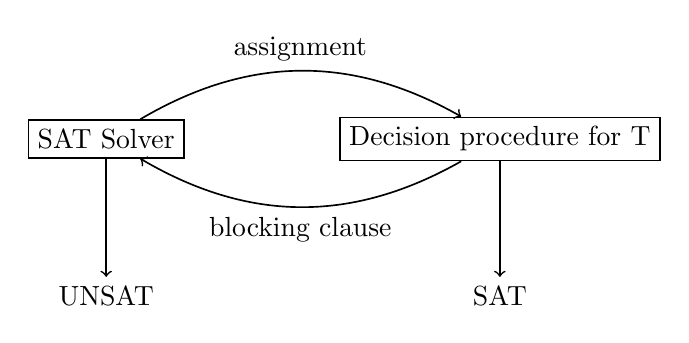
\begin{tikzpicture}[semithick,->,node distance=2cm]
  \node[draw] (ssolver) at (0,0) {SAT Solver};
  \node (unsat) [below of=ssolver] {UNSAT};
  \node[draw] (dp) at (5,0) {Decision procedure for T};
  \node (sat) [below of=dp] {SAT};

  \path (ssolver) edge [bend left] node[above] {assignment} (dp);
  \path (dp) edge [bend left] node[below] {blocking clause} (ssolver);
  \path (ssolver) edge (unsat);
  \path (dp) edge (sat);

  \end{tikzpicture}
  \end{figure}

\end{frame}

\begin{frame}
  \frametitle{DPLL + T: example}
  \[
    a \land (b \lor (c \land \neg b))
  \]
  \begin{center}
  where $a \mapsto (x=y), b \mapsto (x=z), c \mapsto (y=z)$

  \vspace{10pt}
  \begin{figure}
  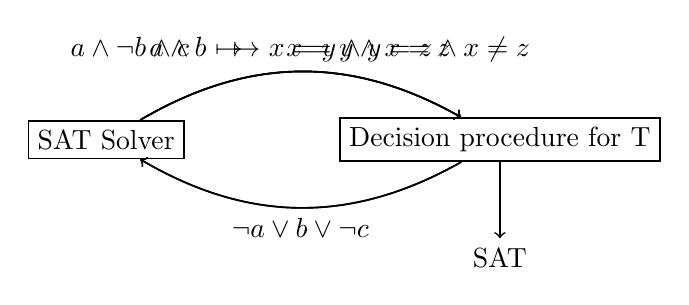
\begin{tikzpicture}[semithick,->,node distance=1.5cm]
  \node[draw] (ssolver) at (0,0) {SAT Solver};
  \node[draw] (dp) at (5,0) {Decision procedure for T};
  \visible<5->{\node (sat) [below of=dp] {SAT};}

  \path (ssolver) edge [bend left] node[above] { } (dp);
  \visible<2>{\path (ssolver) edge [bend left] node[above] {$a \land \neg b \land c ~~\mapsto~~ x = y \land y = z \land x \neq z$} (dp);}
  \visible<4>{\path (ssolver) edge [bend left] node[above] {$a \land b ~~\mapsto~~ x = y \land x = z$} (dp);}
  \path (dp) edge [bend left] node[below] {} (ssolver);
  \visible<3>{\path (dp) edge [bend left] node[below] {$\neg a \lor b \lor \neg c$} (ssolver);}
  \visible<5->{\path (dp) edge (sat);}
  \end{tikzpicture}
  \end{figure}

  \end{center}
\end{frame}
  
\section*{Conclusion}
\begin{frame}
\begin{center}
\Huge
Questions ?
\end{center}
\end{frame}

%TODO

\end{document}
